\documentclass[11pt, a4paper, oneside,UTF8]{article}
\usepackage[UTF8]{ctex}
\usepackage{algorithm}
\usepackage{algorithmic}

\usepackage{geometry}
\geometry{left=3.18cm, right=3.18cm, top=2.54cm, bottom=2.54cm}


\usepackage{graphicx} %插入图片的宏包
\usepackage{float} %设置图片浮动位置的宏包
\usepackage{subfigure} %插入多图时用子图显示的宏包



\title{求一个$N$阶有限群$G$的全部子群}
\author{张子豪\qquad1120203325}
\date{}

\begin{document}

\maketitle

 
\section{循环群}

\subsection{循环群的判断}                       
若$N$为素数,由Lagrange定理的推论,其必为循环群。

若$N$不为素数,由算术基本定理,必有
$$ N=p_{1}^{r_{1}}p_{2}^{r_{2}}\ldots p_{n}^{r_{n}}.$$
其中,$p_{i}$为素数, $r_{i}\in N, i=1,2,3,\ldots ,n$且$p_{1}<p_{2}<\ldots<p_{n}, N>1.$

由第一Sylow定理,$G$中必存在 $p_{i}^{r}$ 阶子群,其中,$1\leq i\leq n$且$1\leq r\leq r_{i}$.

以下考虑 $p_{1}=2$ 且 $r_{1}\geq 2$的情况:

显然,群$G$必存在4阶子群,又Klein四元群是4阶非循环群,故由定理10.14可知,若群$G$存在与Klein四元群同构的子群,则群$G$必为非循环群。

令$G=\{e,a_{1},a_{2},\ldots ,a_{N-1}\}.$
可通过如下算法判断群 $G$ 是否存在子群 $H$ 与Klein四元群同构:

\begin{algorithm}
	\caption{ClienJudge($G,N$)}
	\begin{algorithmic}[1]
		\STATE 找到群$G$的所有二阶元$b_{1},b_{2},\ldots ,b_{s}$
		\IF {$s\leq 2$}
			\RETURN \FALSE
		\ENDIF

		\FOR {$i=1$ to $s-2$}
			\FOR{$j=i+1$ to $s-1$}
				\FOR{$k=j+1$ to $s$}
					\IF{$b_{i}*b_{j}=b_{k}$且$b_{i}*b_{k}=b_{j}$且$b_{j}*b_{k}=b_{i}$}
						\RETURN \TRUE
					\ENDIF
				\ENDFOR
			\ENDFOR
		\ENDFOR
		\RETURN \FALSE
	\end{algorithmic}
\end{algorithm}


若$G$存在与Klein四元群同构的子群,则$G$不是循环群。



\subsection{循环群子群的求解}

若$G$为循环群,根据定理10.14,求解群$G$的所有子群的思路如下:

首先找到群$G$的一个生成元$a$满足$G=<a>$,然后对于$N$的每个正因子$d$,计算$<a^{\frac{n}{d}}>$得到其唯一的$d$阶子群。即求出$G$的所有子群。

算法伪代码如下:

\begin{algorithm}
	\caption{CircleRes($G,N$)}
	\begin{algorithmic}[1]
		\FOR {$i=1$ to $N$}
			\IF {$G=\{a_{i}^1,a_{i}^2,\ldots,a_{i}^N\}$}
				\STATE $a=a_{i}$
			\ENDIF
		\ENDFOR

		\FOR {$d=1$ to $N$}
			\IF {$d|N$}
				\STATE $H=\{a^{n/d},a^{2n/d},\ldots,a^{Nn/d}\}$
				\STATE $print\quad H$
			\ENDIF
		\ENDFOR
	\end{algorithmic}
\end{algorithm}





\section{非循环群}

若$G=\{e,a_{1},a_{2},\ldots ,a_{N-1}\}$为非循环群,不妨设$|a_{1}|\leq |a_{2}|\leq \ldots \leq |a_{N-1}|$ 且 二阶元的数目为$m$,即$a_{1},a_{2},\ldots ,a_{m}$均为二阶元,其中$m\geq 0.$易证$G$中阶大于2的元素个数是偶数,故可将$a_{m+1},a_{m+2},\ldots ,a_{N-1}$表示为$b_{1},b_{2},\ldots ,b_{s},c_{1},c_{2},\ldots ,c_{s}.$ 其中,$c_{i}=b_{i}^{-1}, 2s=N-m-1, i=1,2,\dots ,s.$
即$$ G=\{e,a_{1},a_{2},\ldots ,a_{m},b_{1},b_{2},\ldots ,b_{s},c_{1},c_{2},\ldots ,c_{s}\} $$
所以,对于$G$的某子集$\Omega$,若$\Omega$满足以下条件之一,则$\Omega$一定不是$G$的子群:

(1)$\exists b_{i} \in \Omega,c_{i} \notin \Omega$或
   $\exists c_{i} \in \Omega,b_{i} \notin \Omega$,$i=1,2,\ldots,s.$

(2)$\Omega$中2阶元个数的奇偶性与$|\Omega|$的奇偶性相同

(3)$|\Omega|$ 不是 $N$ 的因子



基于上述分析,可以快速判断某子集$\Omega$不是$G$的子群,由此得到的改进穷举法求解$G$的所有子群的算法如下:


\begin{algorithm}
	\caption{TraverseRes($G,N$)}
	\begin{algorithmic}[1]
		\FOR {$\Omega \in G$}
			\STATE $flag=1,numtwo=0$

			\FOR {$a\in \Omega$}
				\IF {$a*a=e$}
					\STATE $num_two++$
				\ENDIF
			\ENDFOR

			\IF {$numtwo = |\Omega| \bmod 2$ $\lor$ $N\neq |\Omega| \bmod |\Omega|$}
				\STATE $continue;$
			\ENDIF
			
			\FOR {$i\in \{1,2,\ldots,s\}$}
				\IF {$b_{i} \in \Omega \land c_{i} \notin \Omega 
					\lor c_{i} \in \Omega \land b_{i} \notin \Omega$}
					\STATE $flag=0,break;$
				\ENDIF
			\ENDFOR
			
			\IF {$flag=0$}
				\STATE $continue;$			
			\ENDIF

			\FOR {$\forall a,b\in \Omega$}
				\IF{$a*b\notin \Omega$}
					\STATE $flag=0, break;$
				\ENDIF
			\ENDFOR

			\IF {$flag=0$}
				\STATE $continue;$			
			\ENDIF

			\STATE $print\quad \Omega$
		\ENDFOR
	\end{algorithmic}
\end{algorithm}




\section{测试结果}
以Klein四元群为例,结果如图1所示:


\begin{figure}[H] %H为当前位置,!htb为忽略美学标准,htbp为浮动图形
\centering %图片居中
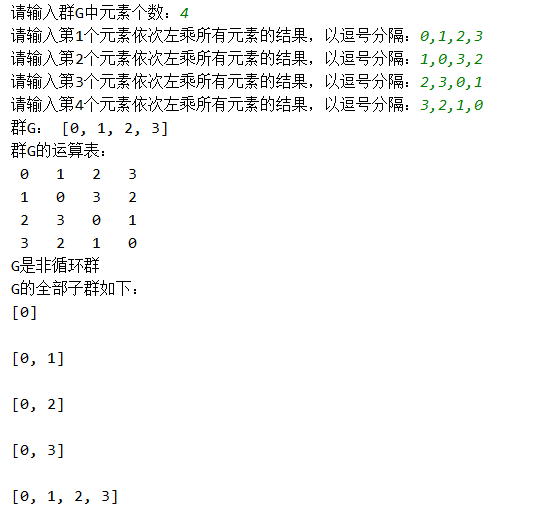
\includegraphics[width=0.7\textwidth]{picture1} %插入图片,[]中设置图片大小,{}中是图片文件名
\caption{} %最终文档中希望显示的图片标题
\label{} %用于文内引用的标签
\end{figure}













\end{document}
